\chapter{Inter-Procedural Dependence Analysis}
\label{ch:interdep}
In the previous chapter we have given detailed explanation of 
heap dependence analysis specified within each procedure. 
This intra-procedural analysis does not cross procedure boundary. 
When the symbolic execution within a procedure reaches a procedure call, 
the analysis approximates the worst case summary for the called 
procedure which conservatively approximates the read and write sets of states 
for the procedure being called. In this chapter we explain how the intra-procedural dependence 
analysis can be extended into a flow sensitive inter-procedural 
analysis. 

Our inter-procedural approach is based on computing 
abstract summary for each procedure at prior. Before analysing the whole program, 
the call graph of the program is preprocessed such that it does 
not contain any recursion. 
The pseudo code outlined in Figure~\ref{fig:interProc} 
gives a top level algorithm of inter-procedural analysis. We 
discuss each step of such analysis in the following 
sections. Section~\ref{sec:callGraph} detects any recursion present 
in the program and processes the call graph accordingly. 
Section~\ref{sec:funcSummary} gives the details of the 
analysis which includes preparing abstract 
summary for each procedure and Section~\ref{sec:interProc} presents 
the technique to effectively use abstract summary of each procedure 
for inter-procedural analysis. 
%
\begin{figure}
%\hrule
\begin{framed}
{\tt
  \begin{program}{0}
  \FL fun interProcAnal(P)  \{
  \UNL{0} G(V, E) = callGraph(P); \COMMENT{G is call graph of program P}
  \UNL{0} \IF (cyclic(G) = TRUE) \COMMENT{Check for recursion}
  \UNL{1} G'(V, E') = findDAG(G); \COMMENT{Transform cyclic graph into DAG}
  \UNL{0} else
  \UNL{1} G' = G;
  \UNL{0} G'' = topologicalSort(G'); \COMMENT{Find topological order of DAG}
  \UNL{0} \FOR each $v_i\in$V following reverse topological order of G'' \{
  \UNL{1} Summary[$v_i$] = findSummary($v_i$);  
  \UNL{0} \COMMENT{Find abstract summary for each procedure}
  \UNL{0} \} 
 % \UNL{8}  \COMMENT{for each function}
  \UNL{0} progAnal(P, Summary); 
  \UNL{0} \COMMENT{Use summaries for inter procedural analysis}
%  \UNL{8} \COMMENT{inter procedural analysis}
  \UNL{-1} \}
  \end{program}
}
\end{framed}
%\hrule
  \caption{Top level algorithm for inter-procedural analysis\label{fig:interProc}}
%\hrule  
\end{figure}
%
\section{Processing and Ordering of Call Graph}
\label{sec:callGraph}
Our inter-procedural analysis works on call graph of the 
program under analysis. Call graph \emph{G}(\emph{V}, \emph{E}) 
is a directed graph that represents calling relationships 
between caller and callee procedures. Specifically, each 
node $v_i\in$ \emph{V} represents a procedure and each directed 
edge (\emph{f}, \emph{g})$\in$ \emph{E} indicates that procedure 
\emph{f} calls procedure \emph{g}. Thus, a cycle in the graph indicates 
recursive procedure calls. 

Our approach needs to transform the cyclic call graph into directed 
acyclic graph (DAG) for efficient computation of abstract summary. 
The call graph without any recursion is always DAG. To transform cyclic 
directed call graph into DAG, the back edges 
from the cyclic graph are removed and a summary node is introduced. This 
summary node approximates all the remaining levels of recursion and 
abstracts the worst case summary of the functions present in the recursion. 
The nodes of directed acyclic call graph, thus obtained, are ordered using 
topological sort. Each node in the acyclic call graph will be assigned a sequence 
order following which the procedures are processed. 
\begin{figure}
  \begin{center}
 
    \scalebox{.85}{\begin{tabular}{| c c |}
     \hline
     {\tt
\begin{program}{0}
%  \FL\ \ldots
  \NL{0} procedure f() 
  \NL{0} begin
  \NL{2}  call g();
  \NL{2}  call h();
  \NL{0}  end
  \NL{0} procedure g()
  \NL{0}  begin
  \NL{2}     call k();
  \NL{0}  end
 \end{program}
 
} %\cline{1-1}
     &
      {\tt
\begin{program}{9}
 \NL{0}  procedure k()
   \NL{0}  begin
   \NL{2}  call g();
   \NL{0}  end
    \NL{0}  procedure h()
    \NL{0}  begin
    \NL{2}  call i();
    \NL{2}  call j();
    \NL{0}  end
\end{program}
 
} \\
%      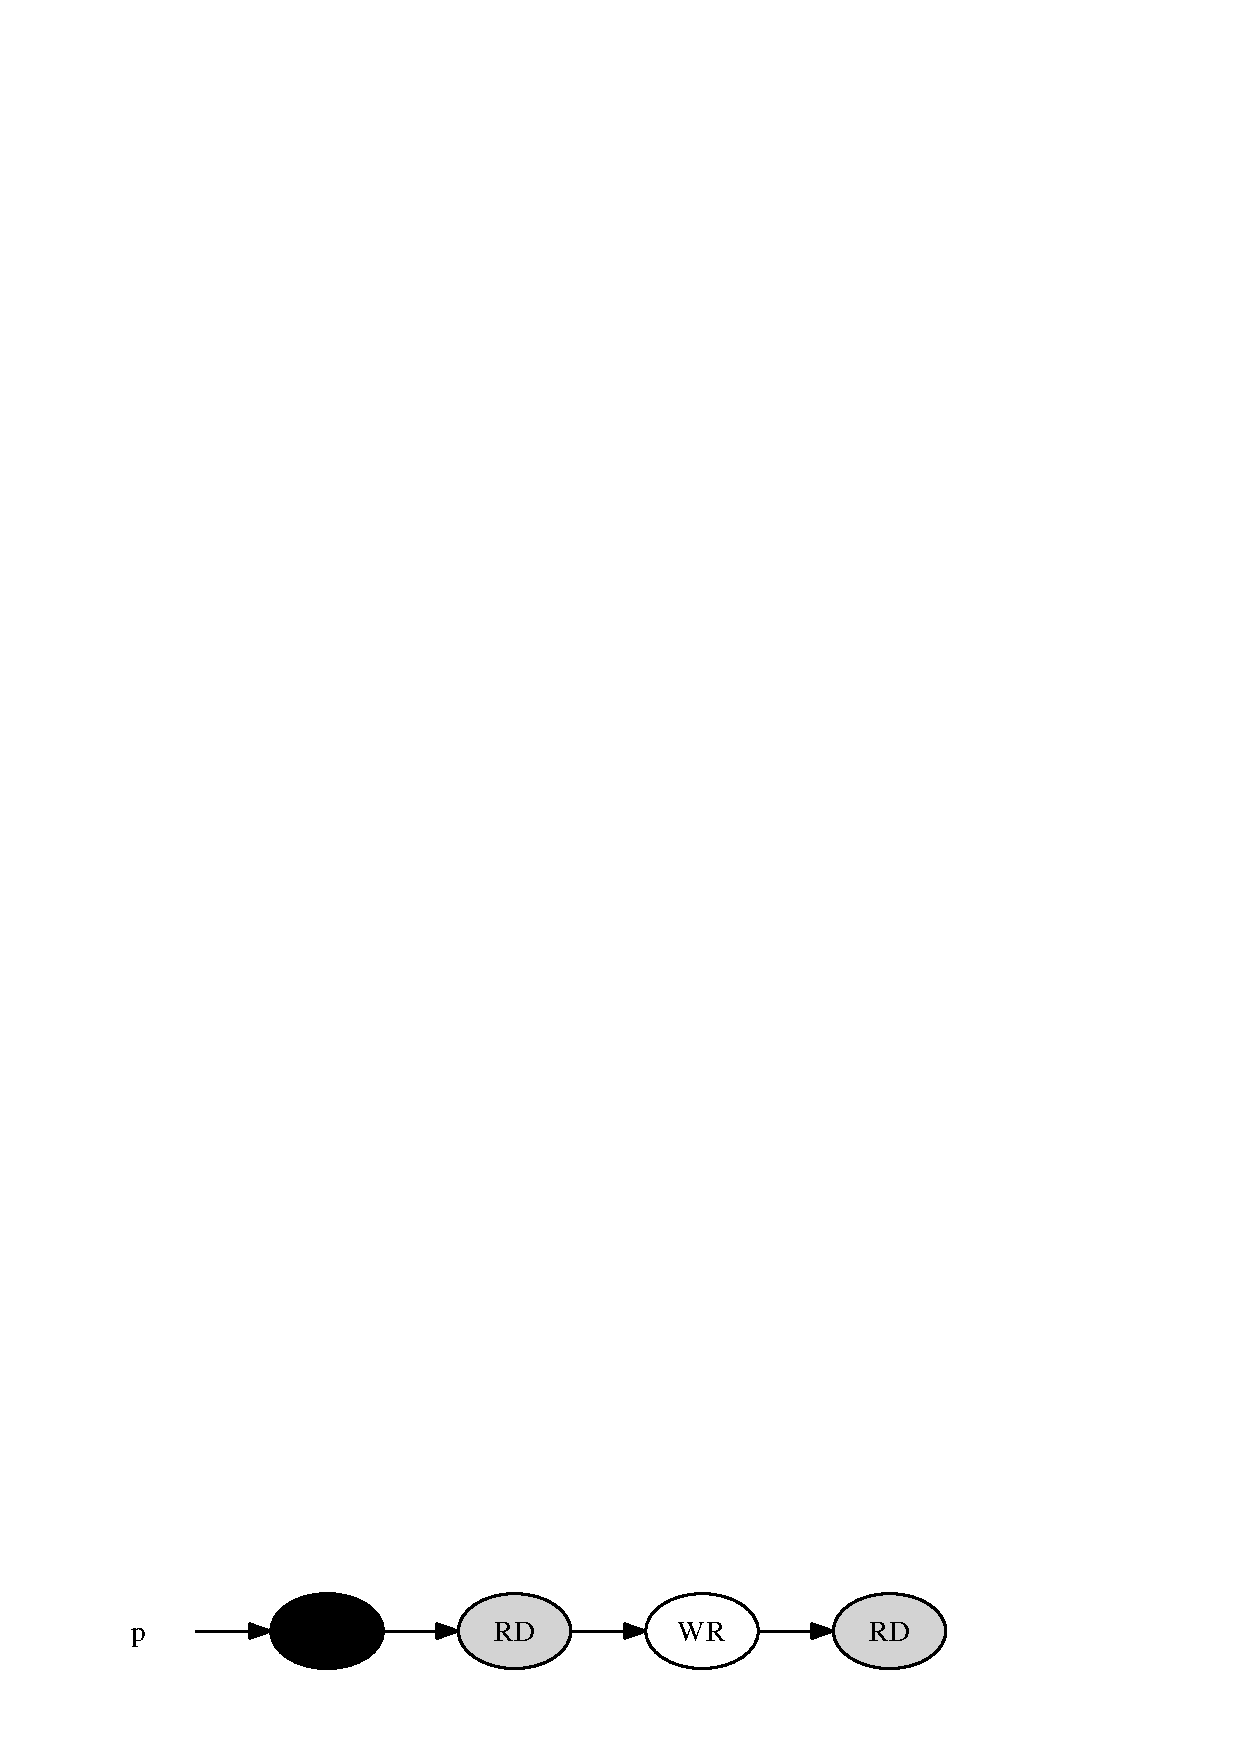
\includegraphics[scale=0.6]{grph_RD_WR} & \\
%      (a) & (b) \\
  %    (a) Nodes read and written by code & 
  %    (b) Code fragment traversing the data structure. \\
  \hline
    \end{tabular}}
  \end{center}
%  \hrule
  \caption{\label{fig:codeCallGraph} Skeleton of a program with procedure calls}
%\hrule
\end{figure}
  
\begin{example}{\rm
Consider the program shown in Figure~\ref{fig:codeCallGraph}. In this example 
procedure \ttf{f} calls procedure \ttf{g} and procedure \ttf{h}, whereas, 
procedure \ttf{h} again calls procedures \ttf{i} and \ttf{j}. Procedure \ttf{g} calls 
procedure \ttf{k} which in turn calls procedure \ttf{g}, resulting in 
indirect recursive procedure calls. Figure~\ref{fig:callgraph}(a) shows the corresponding 
directed call graph. The shadowed cyclic region in the graph indicates recursion 
in the program. The cyclic call graph is then 
transformed into acyclic graph by removing the 
back edge showed as dotted edge. Figure~\ref{fig:callgraph}(b) presents 
corresponding acyclic graph 
with topological order. 
}
\hfill\psframebox{}  \end{example}
%
\section{Computing Abstract Summary}
\label{sec:funcSummary}
For each callee procedure, we need to obtain 
an abstract summary that summarizes the procedure. 
By abstract summary, we mean the \emph{Read} 
and \emph{Write} sets of symbolic heap locations which are accessed 
for reading and writing operations respectively inside the procedure. 
The motivation behind the technique is to summarize effect of called 
procedure for callers, which in turn is used by the callers to summarize effect 
for called procedure. Summaries, thus obtained for 
each procedure are stored in a table for later use. In  
this analysis propagation of summaries 
follows the bottom-up approach. Hence, abstract summary for all the 
procedures are computed following the reverse topological order of nodes in the 
call graph. 
\begin{figure}
  \begin{center}
    \scalebox{.85}{\begin{tabular}{ c c }
     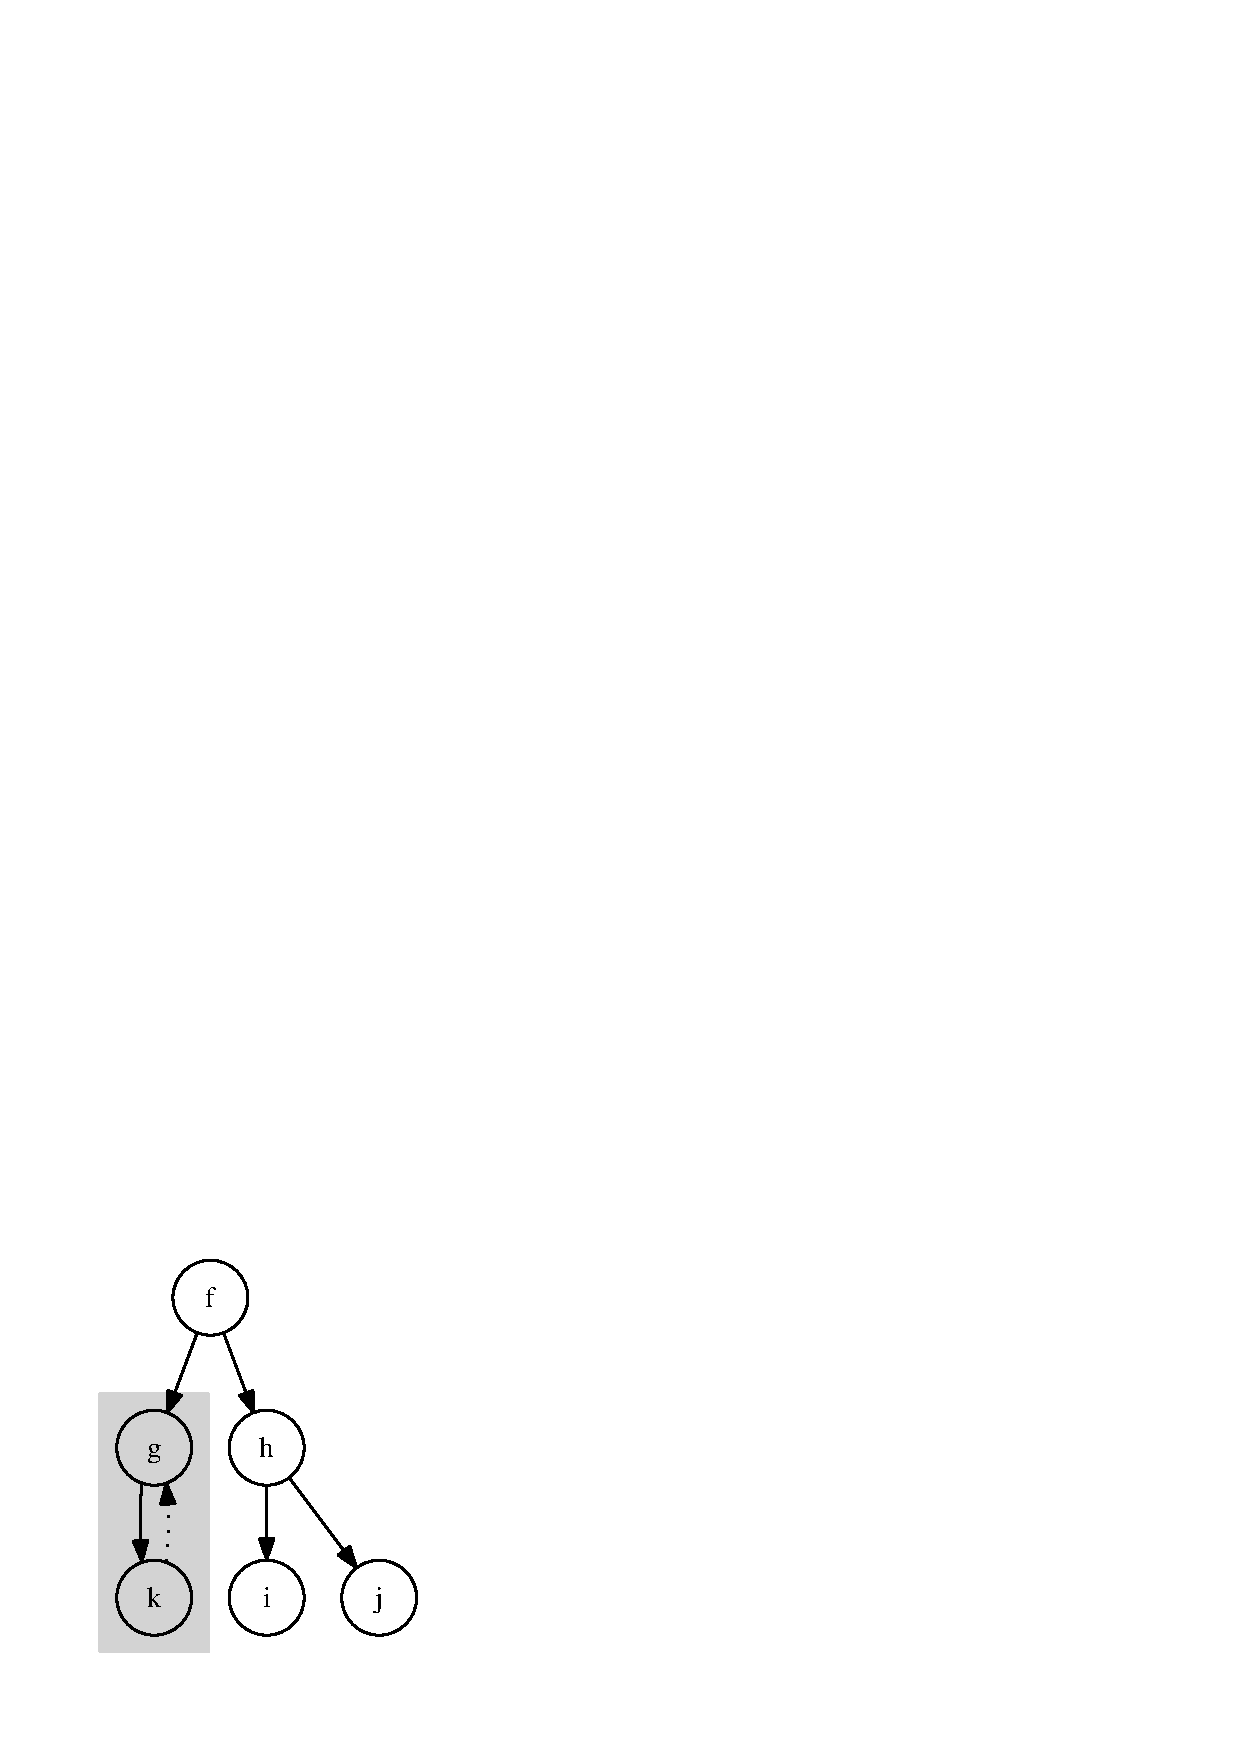
\includegraphics[scale=0.75]{call_graph} %\cline{1-1}
     &
      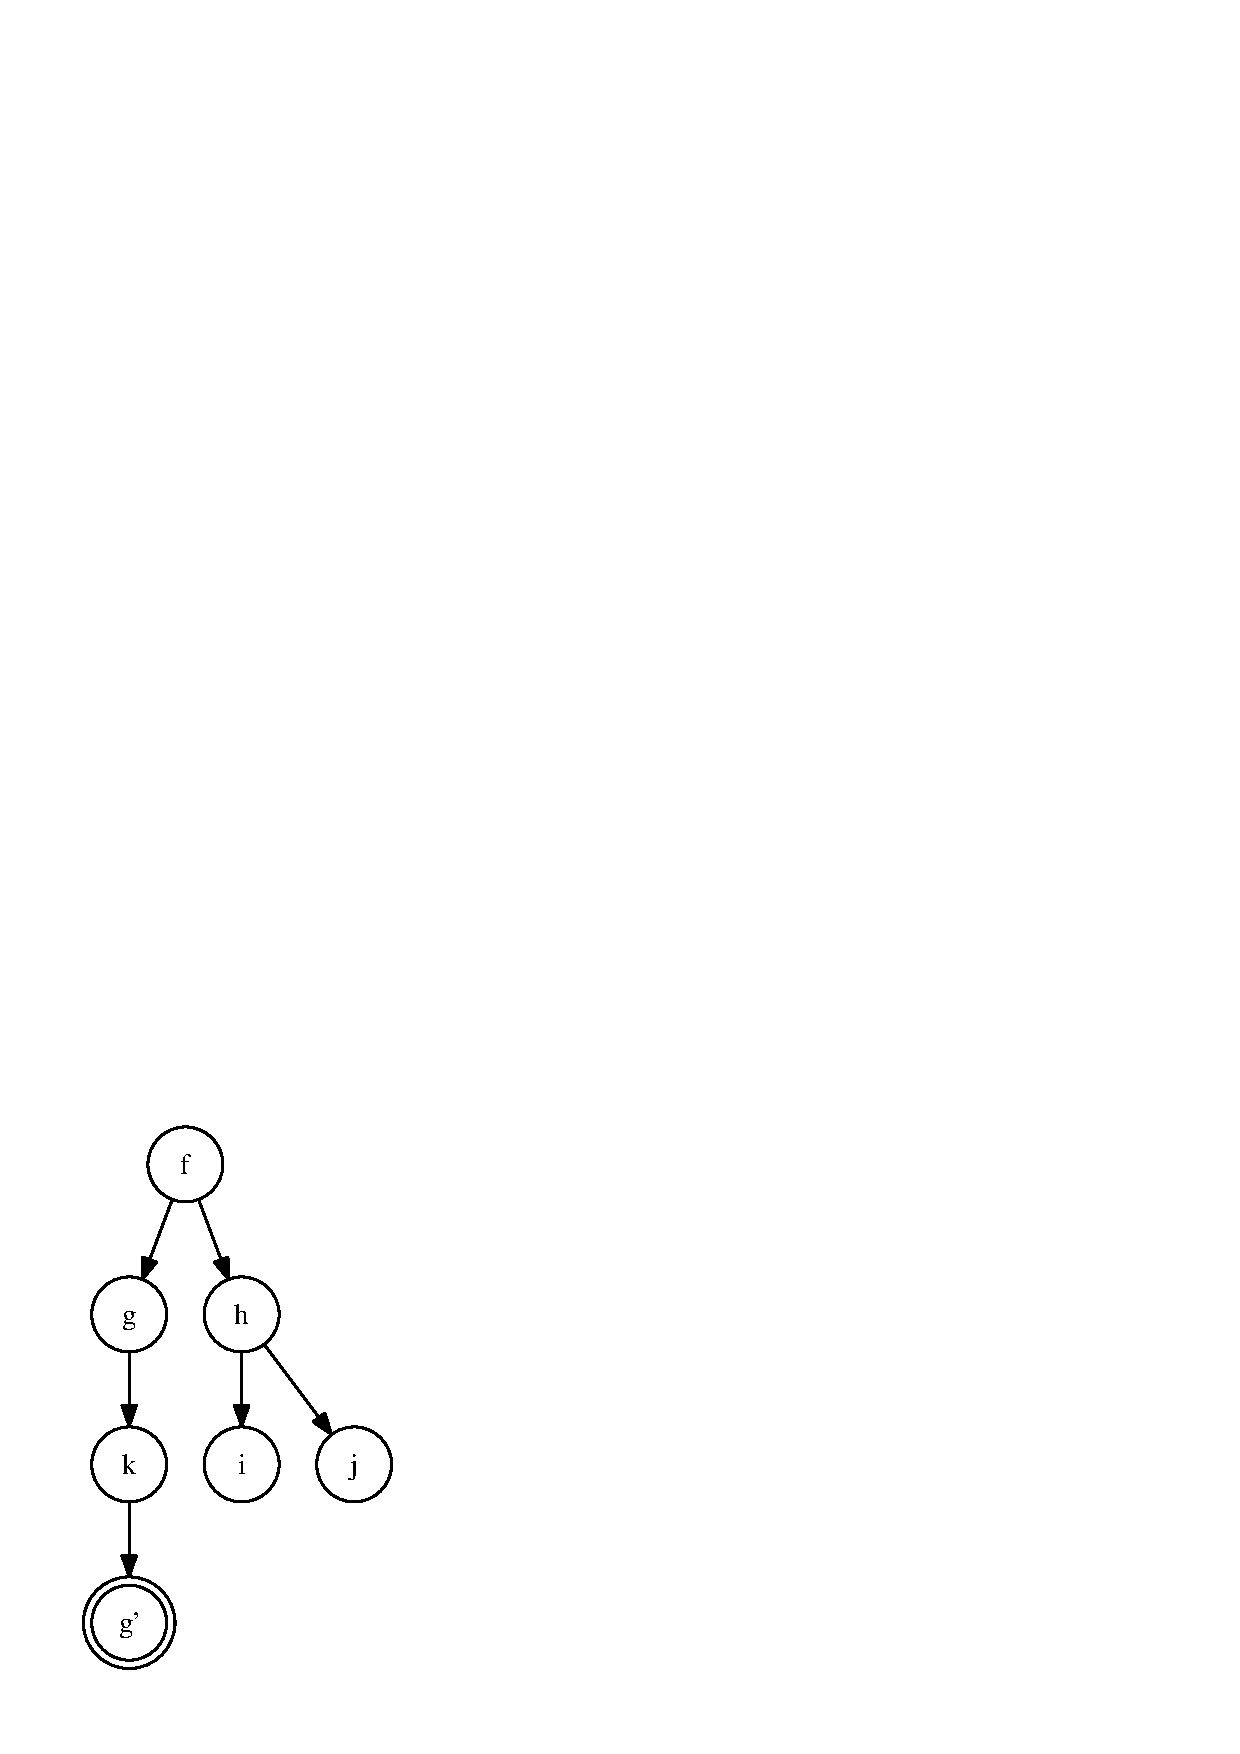
\includegraphics[scale=0.75]{ordered_graph} \\
%      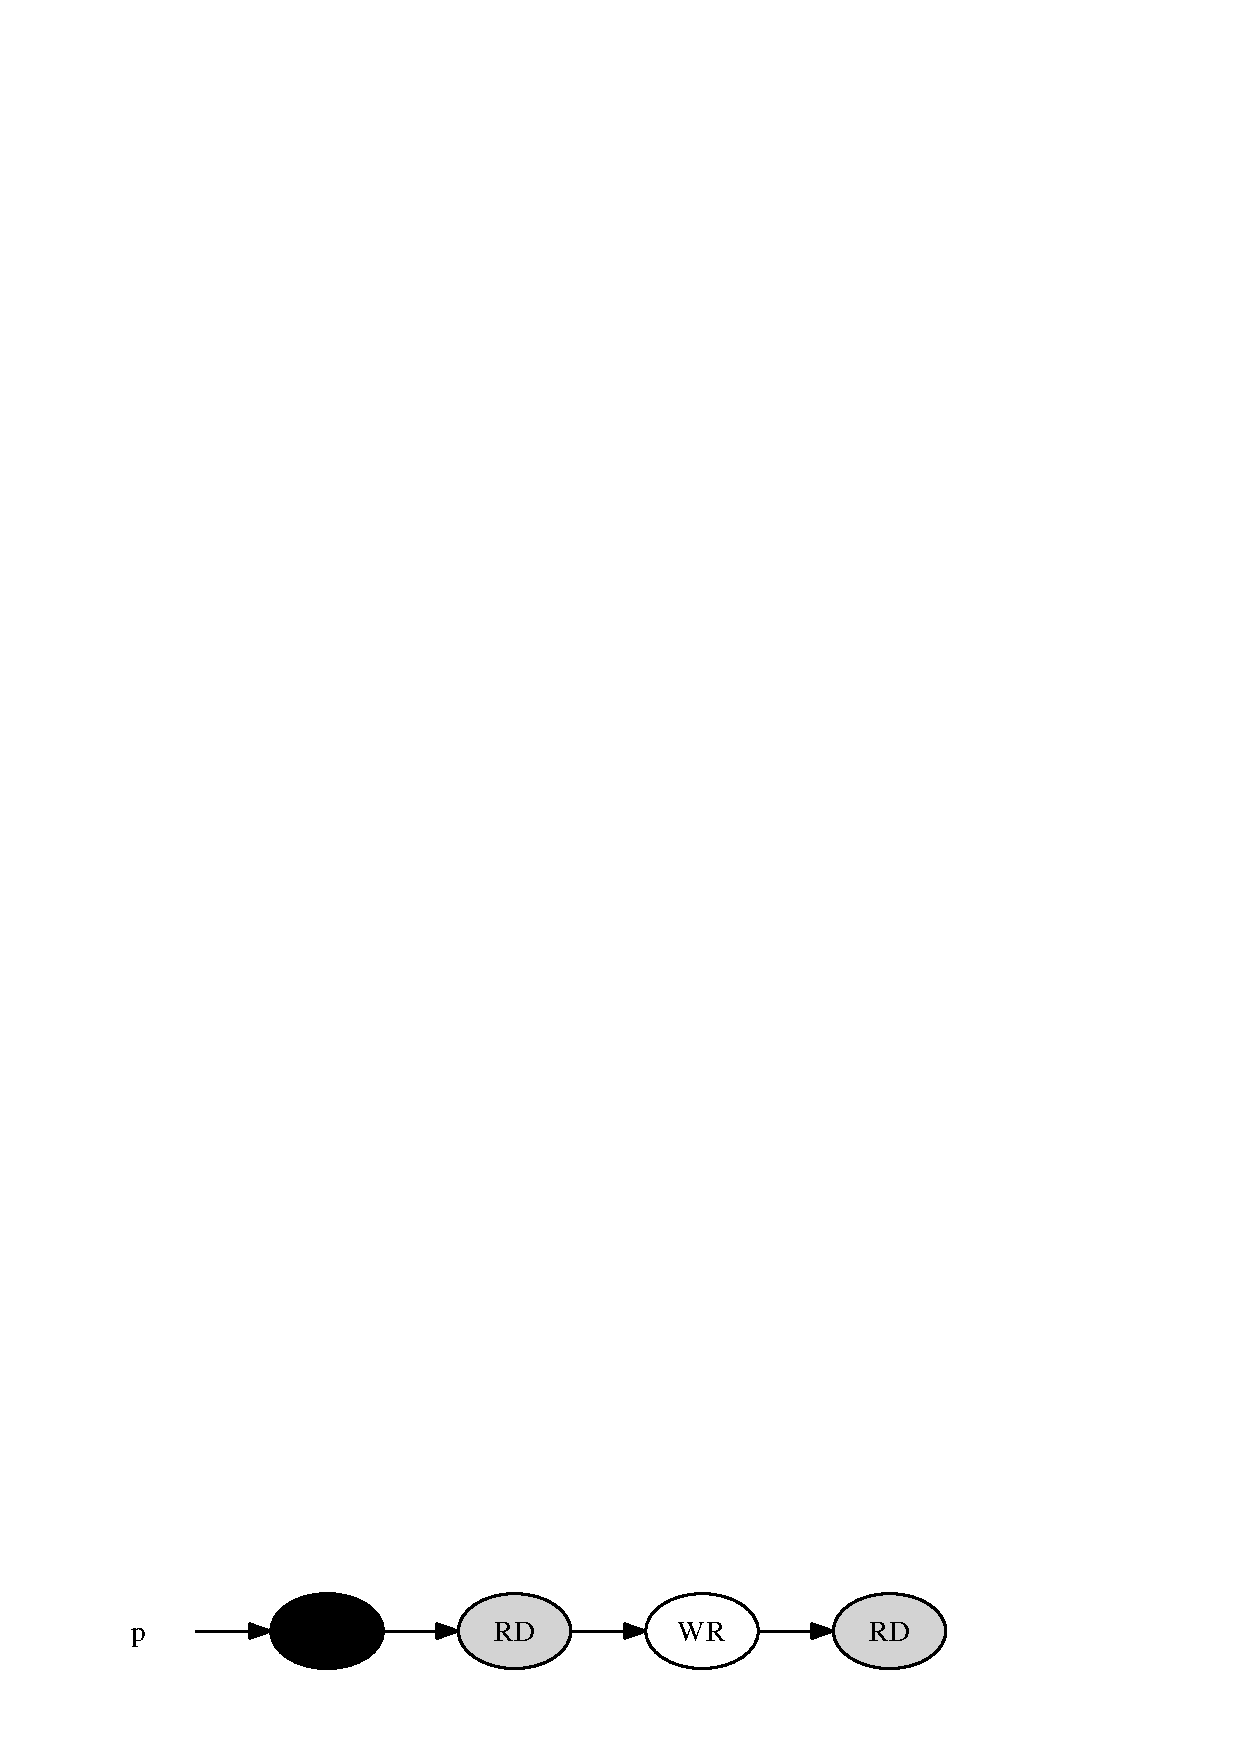
\includegraphics[scale=0.6]{grph_RD_WR} & \\
%      (a) & (b) \\
     (a) Cyclic call graph & 
     (b) Corresponding DAG \\
    \end{tabular}}
  \end{center}
%  \hrule
  \caption{\label{fig:callgraph} Example showing call graph }
%\hrule
\end{figure}
  
All heap directed global  
pointer variables throughout the program are initialized once with proper 
symbolic memory locations. During computation of abstract summary for each  
procedure, the heap directed pointer variables passed as formal 
parameters to the called procedure are 
initialized with random symbolic memory location. As summary, 
our analysis computes read and write sets of access paths with respect 
to the corresponding symbolic memory locations. This process of computation 
follows the intra-procedural analysis as explained before. The same 
procedure is followed by the caller procedure to summarize its effect. 
%
\section{Evaluating Procedure Call}
\label{sec:interProc}
Abstract summary for each callee procedure should be 
used by the caller procedure in the current calling context. 
Summary of each called procedure, thus obtained by intra-procedural analysis, 
contains information in the local context of the procedure.
When the symbolic execution inside the caller function reaches a procedure call, 
the context of the actual parameters is mapped to the respective 
formal parameters of the called procedure. The summary of the callee is 
translated accordingly to be used in the context of caller procedure. 

Summary of a procedure, as mentioned earlier, returns read and write sets 
of paths accessed by corresponding pointer variables. Access paths 
are computed with respect to symbolic memory locations local to the callee  
under analysis. The local symbolic memory locations used in the 
summary of callee are 
mapped into symbolic locations accessed by the caller procedure. 
Such modified summary of caller is used by the callee to summarize its effect. 
Evaluating summary for recursive function does not differ significantly than evaluating non-recursive function. If a recursive function is encountered, the 
analysis will go deep inside the function upto the depth of recursion depending 
upon the precision of analysis. 
\begin{figure}[t]
  \begin{center}
    \scalebox{.85}{\begin{tabular}{ c | c }
%    \hline
	 \multirow{2}{*}{{\tt
\begin{program}{0}
%  \FL\ \ldots
  \NL{0} procedure f(p) 
  \NL{0} begin
  \NL{1}  q = p\rtarrow{next};
  \NL{1}  g(q);
  \NL{0}  end
  \NL{0} procedure g(r)
  \NL{0}  begin
  \NL{1}  $\cdots$ = r\rtarrow{num};
  \NL{1}  s = r\rtarrow{next};
  \NL{1}  s\rtarrow{num}=$\cdots$;
  \NL{0}  end
 \end{program}
 
}} %\cline{1-1}
     & \\
    & 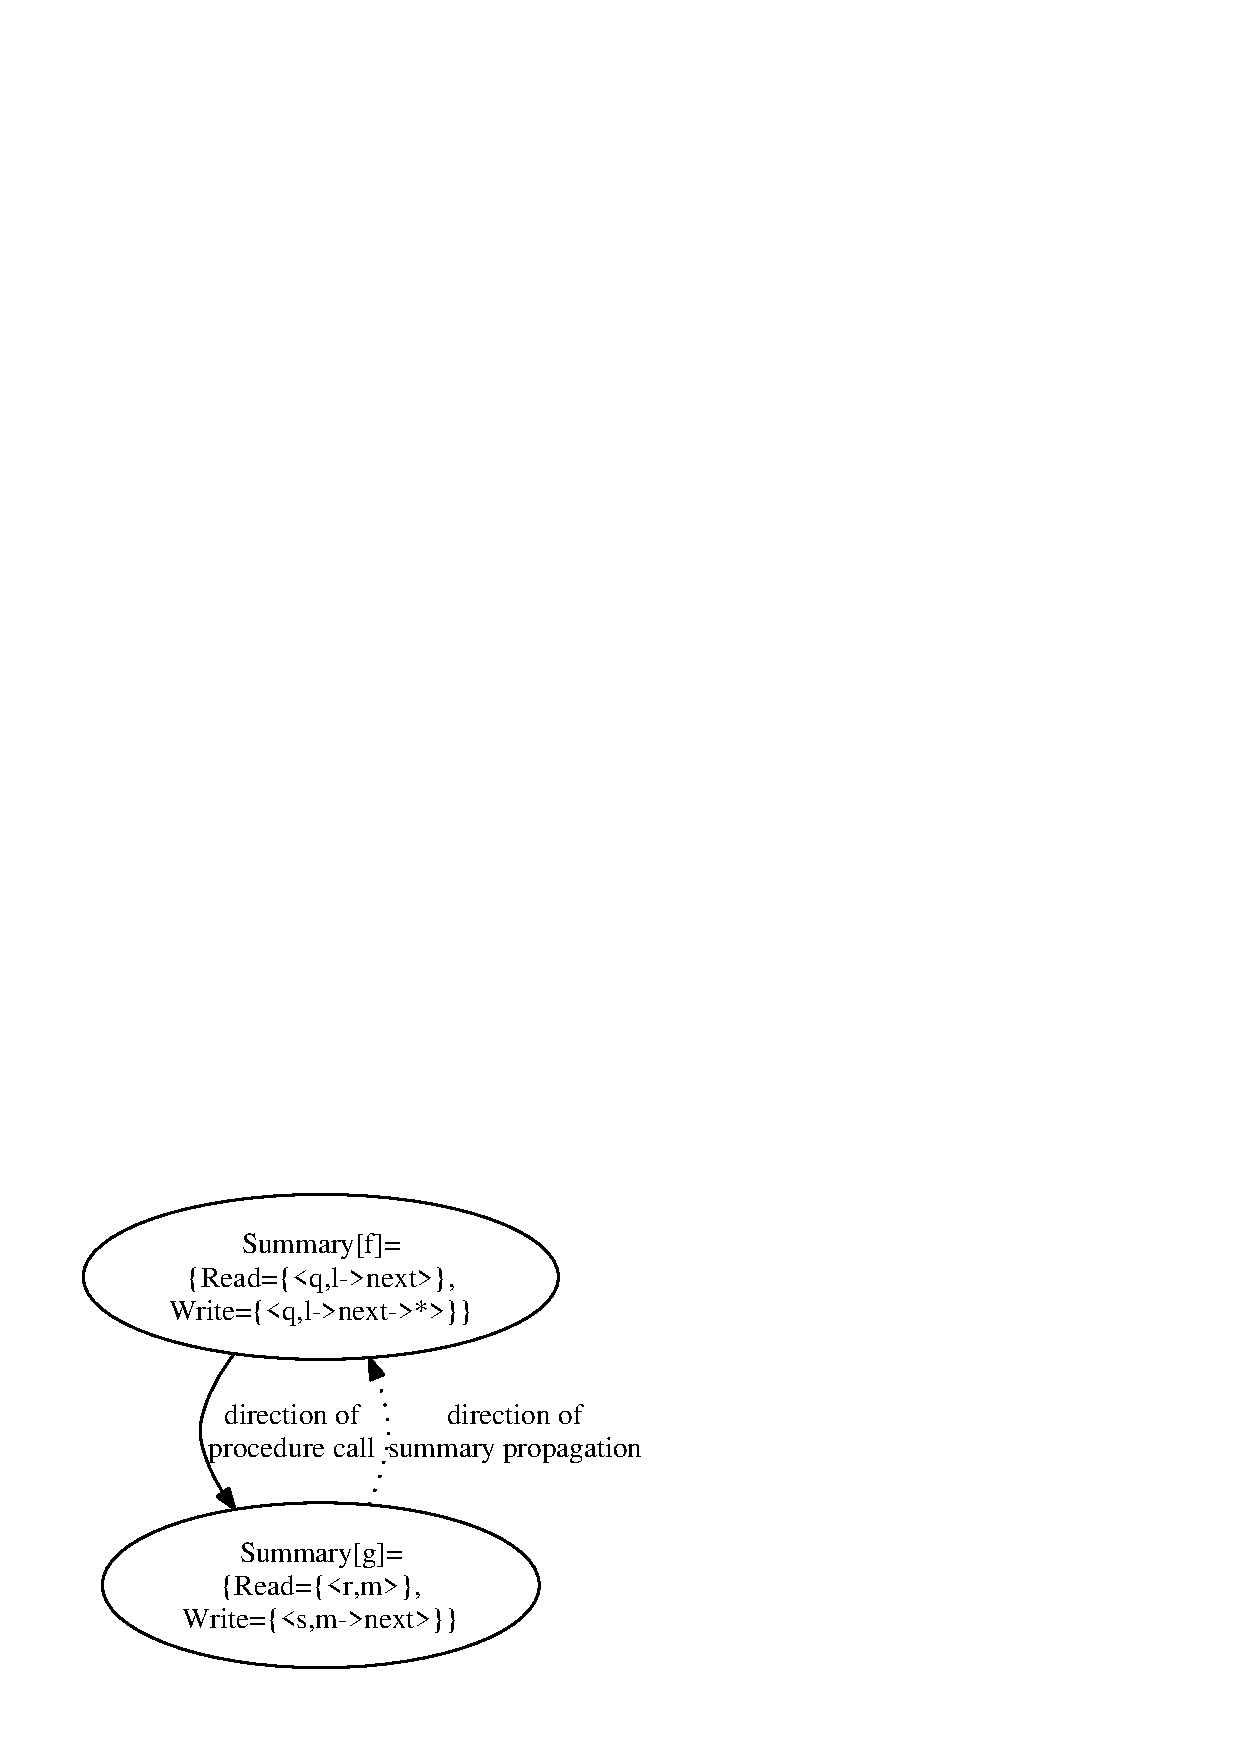
\includegraphics[scale=0.7]{grph5} \\
%      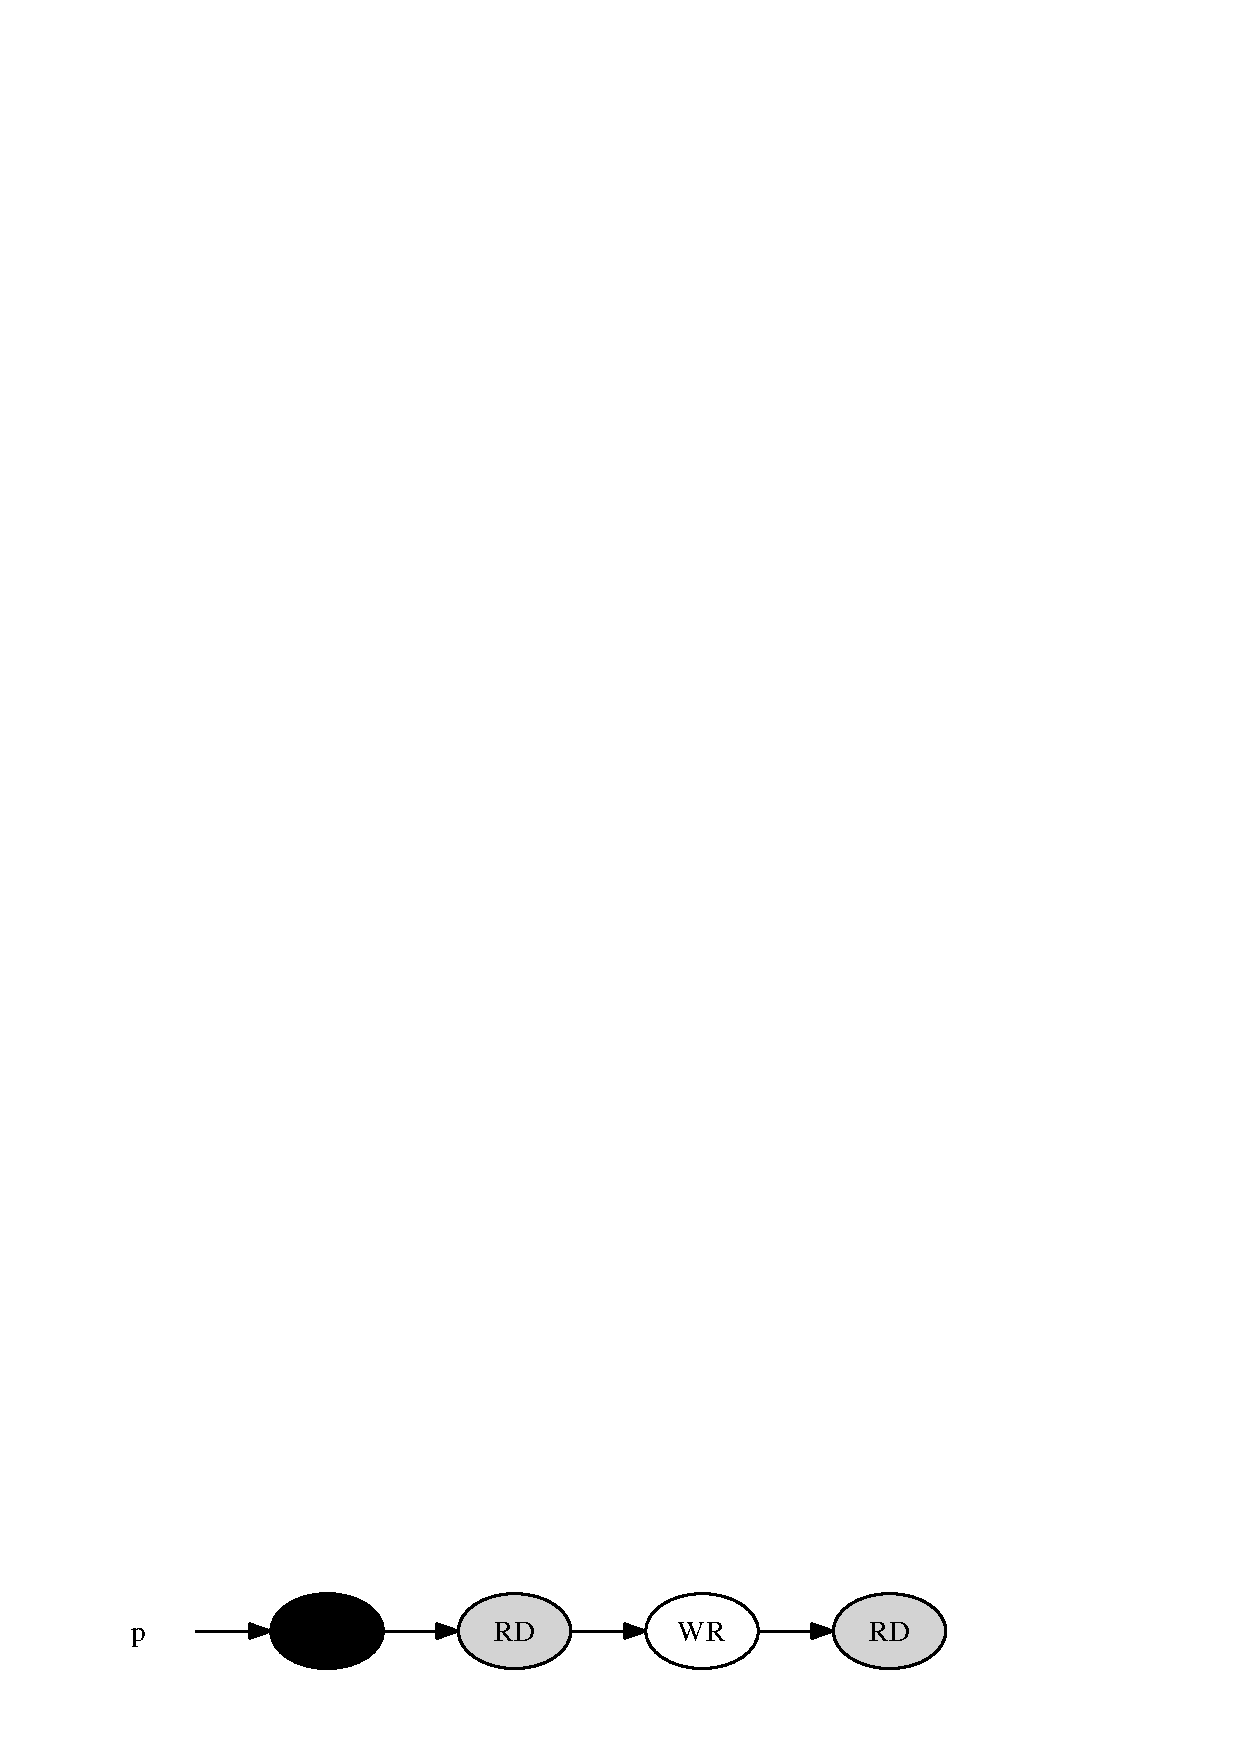
\includegraphics[scale=0.6]{grph_RD_WR} & \\
%     (a) & (b) \\
      (a) Example program with procedure call &
     (b) Call graph showing summary of procedures \\
 %    \hline
%     \hline
    \end{tabular}}
  \end{center}
  \hrule
  \caption{\label{fig:codeInter} Example showing computation of abstract summary}
%\hrule
\end{figure}
\begin{example}{\rm 
Let us consider the example program and the corresponding call graph shown in 
Figure~\ref{fig:codeInter}. In the example program procedure 
\ttf{f} calls procedure \ttf{g}. The solid line in the call graph gives the direction 
for calling subroutines, whereas, the dotted line shows the direction for propagation 
of summary information. Summary information of procedure \ttf{f} and \ttf{g} are also shown in the call graph. At first, summary of procedure \ttf{g} is computed in the 
local context of itself. The summary consists of read and write sets as 
\ttf{\{<r,m>\}} and \ttf{\{<s,m\rtarrow{next}>\}} respectively, where pointer 
variable \ttf{r} is initialized to symbolic memory location \ttf{m}. 
At the call site of procedure \ttf{g}, the actual parameter \ttf{q} takes value 
\ttf{l\rtarrow{next}}, if formal parameter \ttf{p} of procedure \ttf{f} 
points to memory location \ttf{l}. The value of actual parameter \ttf{q} 
modifies the summary of procedure \ttf{g}. This modified summary is further used 
to summarize the information of procedure \ttf{f}. 

}
\hfill\psframebox{}    
\end{example}












